\documentclass[conference,10pt]{IEEEtran}
 \IEEEoverridecommandlockouts
\usepackage{cite}
\usepackage{color}
\usepackage[pdftex]{graphicx}
\graphicspath{{fig/}{jpeg/}}
\usepackage[cmex10]{amsmath}
\usepackage{amssymb}
\usepackage{algorithm}
\usepackage{algorithmic}
\usepackage{subcaption}
\usepackage[outdir=./]{epstopdf}
%\usepackage{algpseudocode}
\usepackage{hyperref}
\usepackage{comment}
\input{../mysymbol.sty}
\input{../my_sections.tex}
\usepackage{tikz}
\usetikzlibrary{shapes,arrows}
\usepackage{float,environ}
\usetikzlibrary{matrix} % for block alignment
\usetikzlibrary{decorations.markings} % for arrow heads
\usetikzlibrary{calc} % for manimulation of coordinates
\usetikzlibrary{decorations.pathmorphing,snakes, positioning, decorations.pathreplacing}

\usetikzlibrary{fit}
%\input{figures/tikh_styles}

\usepackage{pgfplots}
\usepackage{color}
%\usepackage{setspace}
%\usepackage{hyperref}
\usepackage{multirow}
%\usepackage{rotating}
%\usepackage{comment}
%\usepackage{flushend}
%\usepackage{caption}
%\usepackage{subcaption}
%\usepackage[affil-it]{authblk}
%\usepackage{bm}
%\usepackage{algorithm}
%\usepackage{algorithmic}
%\usepackage{enumerate}
%\usepackage{morefloats}
%\usepackage{setspace}

\makeatletter
\newsavebox{\measure@tikzpicture}
\NewEnviron{scaletikzpicturetowidth}[1]{%
  \def\tikz@width{#1}%
  \def\tikzscale{1}\begin{lrbox}{\measure@tikzpicture}%
  \BODY
  \end{lrbox}%
  \pgfmathparse{#1/\wd\measure@tikzpicture}%
  \edef\tikzscale{\pgfmathresult}%
  \BODY
}
\makeatother

\newcommand{\QED}{\hfill\ensuremath{\blacksquare}}
\newcommand{\norm}[1]{\ensuremath{\left\| #1 \right\|}}

%\IEEEoverridecommandlockouts 
\def \vneg {\vspace{-.5cm}}

\def\whp{\text{w.h.p}}
\def\E{\mathbb{E}}
\def\P{\mathbb{P}}
\def\supp{\text{support}}
\def\Tr{\text{Tr}}
\def\vec2{\text{vec}}


% Resource allocation functions
\def \fph  {\bbf\big(\bbp(\bbh), \bbh\big)}
\def \Efph {\mbE\big[\fph\big]}
%
% Optimal power allocation functions
\def \fphstar  {\bbf\big(\bbp^*(\bbh),\bbh\big)}
\def \Efphstar {\mbE\big[\fphstar\big]}
%
% Slater's condition power allocation functions
\def \fphzero  {\bbf\big(\bbp_0(\bbh),\bbh\big)}
\def \Efphzero {\mbE\big[\fphzero\big]}
%
% Parametrized power allocation functions
\def \fphih  {\bbf\big(\bbphi(\bbh,\bbtheta),\bbh\big)}
\def \Efphih {\mbE\big[\fphih\big]}
%
% Parametrized power allocation functions indexed by sample index k
\def \fpihk {\bbf\big(\bbh_k,\bbphi(\bbh_k,\bbtheta_k)\big)}
%
% Lagrangian
\def \Lagphi {\ccalL_{\bbphi}(\bbtheta,\bbx, \bblambda, \bbmu)}


%\addtolength{\textwidth}{10mm}
%\addtolength{\evensidemargin}{-5mm}
%\addtolength{\oddsidemargin}{-5mm}
%\addtolength{\textheight}{10mm} 
%\addtolength{\topmargin}{-5mm}

%\renewcommand \blue[1]{}  \renewcommand \red[1]{}   

\newtheorem{assumption}{\hspace{0pt}\bf Assumption}
\newtheorem{lemma}{\hspace{0pt}\bf Lemma}
\newtheorem{proposition}{\hspace{0pt}\bf Proposition}
\newtheorem{example}{\hspace{0pt}\bf Example}
\newtheorem{observation}{\hspace{0pt}\bf Observation}
\newtheorem{theorem}{\hspace{0pt}\bf Theorem}
\newtheorem{corollary}{\hspace{0pt}\bf Corollary}
\newtheorem{fact}{\hspace{0pt}\bf Fact}
\newtheorem{remark}{\hspace{0pt}\bf Remark}
\newtheorem{test}{\hspace{0pt}\it Test Case}
\newtheorem{definition}{\hspace{0pt}\bf Definition}
\newtheorem{conj}{\hspace{0pt}\bf Conjecture}




% Title.
% ------
\begin{document} 
%
% Single address.
% ---------------

\title{Primal-Dual Learning for Resource Allocation \\ in Low Latency Wireless Systems}
\author{Mark Eisen$^*$ \quad Mohammad M. Rashid$^\dagger$ \quad 
			Dave Cavalcanti$^\dagger$ \quad Alejandro Ribeiro$^*$
\thanks{{Supported by Intel Science and Technology Center for Wireless Autonomous Systems. The authors are with the $(*)$Department of Electrical and Systems Engineering, University of Pennsylvania and $(\dagger)$Wireless Communications Research, Intel Corporation. Email: maeisen@seas.upenn.edu, mamun.rashid@intel.com, dave.cavalcanti@intel.com, aribeiro@seas.upenn.edu}.}}


\maketitle

%\thispagestyle{empty}
%
\begin{abstract}
We consider the problem of scheduling transmissions over low-latency wireless communication links to control various control systems. Low-latency requirements are critical in developing wireless technology for industrial control, but are inherently challenging to meet while also maintaining reliable performance. An alternative to ultra reliable low latency communications (URLLC) is a framework in which reliability is adapted to control system demands. We formulate the control-aware scheduling problem as a constrained statistical optimization problem in which the optimal scheduler is a function of current control and channel states. The scheduler is parameterized with a deep neural network, and the constrained problem is solved using techniques from primal-dual learning. Furthermore, these updates are model-free in that they do not require explicit knowledge of channels models or performance metrics. The resulting control-aware deep scheduler is evaluated in empirical simulations and strong performance is shown relative to other heuristic scheduling methods.
\end{abstract}
%

\begin{IEEEkeywords}
wireless control, low-latency, deep learning, primal-dual
\end{IEEEkeywords}


\section{Introduction}

The recent advances in wireless technology and automation have given rise to efforts in integrating wireless communications in autonomous environments, particularly in industrial control settings where the scale of wired networks is proving increasingly costly \cite{zand2012wireless, wollschlaeger2017future}. The analysis of control systems operating over wireless communication links is thus an integral apart in enabling these wireless industrial automation applications. However, the performance specifications of these applications demands the design of wireless networks that can meet both the high reliability and low latency demands of the system \cite{zand2012wireless, varghese2014wireless, weiner2014design, popovski2018wireless, bennis2018ultra}. The problem of ultra reliable low latency communications (URLLC) is inherently challenging as the physical medium of wireless communication trades off these two performance criteria, making it hard to meet both reliability and latency demands.

One promising direction in enabling low latency communications involves specific developments in radio resource allocation, or scheduling. For low latency applications, traditional delay-aware schedulers ~\cite{wu2014analysis, lu1999fair, andrews2001providing} have been employed, in addition to more recent URLLC techniques based on various forms of diversity \cite{swamy2015cooperative, popovski2018wireless, nielsen2018ultra, ashraf2018dynamic}---all of which are agnostic to the control system. However, due to the physical limitations of the wireless channel, it is often necessary to use information from the control system to make proper use of scheduling resources in meeting latency requirements. While there exist numerous ways in which control system information is incorporated into ``control-aware'' scheduling methods \cite{Cervin_event_scheduling, mamduhi2014event,shi2011optimal,han2017optimal, GatsisEtal15,demirel2018deepcas,leong2018deep}, these are agnostic to latency requirements of the system. More recent work \cite{eisen2018control} looks at heuristic based scheduling methods that are both control and latency aware. 

Aside from traditional heuristic based scheduling methods, tools from machine learning are being incorporated into making intelligent scheduling and resource allocation decisions. The work in \cite{eisen2018learninga} builds a framework for solving a generic set of resource allocation problems by interpreting resource allocation as a constrained statistical learning problem. This leads a natural use of learning models, such as deep neural networks (DNNs), for designing schedulers. Recent advancements apply techniques from both reinforcement learning and deep learning for control-aware scheduling in simple systems \cite{demirel2018deepcas,leong2018deep}. The goal in this work is to use the framework of \cite{eisen2018learninga} to employ so-called primal-dual deep learning to tackle develop novel scheduling techniques that are both control-aware and latency constrained. 

This paper is organized as follows. We formulate the wireless control system in which state information is communicated to the control over a wireless channel as a switched dynamical system (Section \ref{sec_problem}). We further discuss the scheduling architecture under which we can allocate channels and data rates between plants. With this formulation, we formulate the optimal scheduling problem that minimizes a control cost under latency constraints (Section \ref{sec_opt}). As this problem is a statistical learning problem, it can be parameterized with a deep neural network (Section \ref{sec_param}). To handle the constraints, we convert the problem to the Lagrangian dual problem and present a primal-dual learning method to find the optimal parameters (Section \ref{sec_primal_dual}). We further discuss ways in which the primal-dual method can be approximated without explicit model knowledge (Section \ref{sec_model_free}). The performance of the learned control-aware scheduling method is analyzed in a numerical simulation of a control system with latency constrained and compared other heuristic scheduling methods (Section \ref{sec_numerical_results}). 



%\input{Problem_formulation_icassp}

\section{Wireless Control Systems}\label{sec_problem}

%
\begin{figure}
\centering
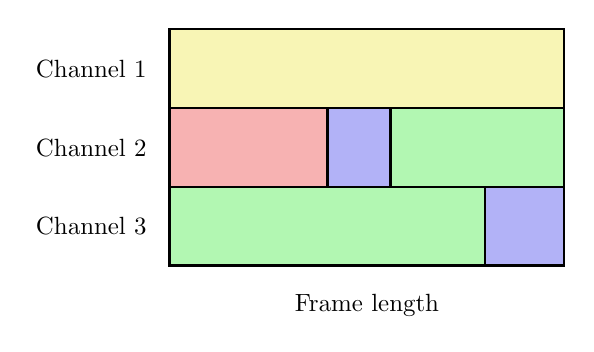
\begin{tikzpicture}
\draw[black,very thick] (-4,-1) rectangle (1,0);
\draw[black,very thick] (-4,0) rectangle (1,1);
\draw[black,very thick] (-4,1) rectangle (1,2);
\draw [step=.3, thick, draw= black, fill=black!10!green!30] (-4,-1) rectangle  (0,0);
\draw [step=.3, thick, draw= black, fill=black!10!blue!30] (0,-1) rectangle  (1,0);
\draw [step=.3, thick, draw= black, fill=black!10!red!30] (-4,0) rectangle  (-2,1);
\draw [step=.3, thick, draw= black, fill=black!10!blue!30] (-2,0) rectangle  (-1.2,1);
\draw [step=.3, thick, draw= black, fill=black!10!green!30] (-1.2,0) rectangle  (1,1);
\draw [step=.3, thick, draw= black, fill=black!10!yellow!30] (-4,1) rectangle  (1,2);
\node[align=center, scale =0.9] at (-1.5,-1.5) {Frame length};
\node[align=center, scale =0.9] at (-5,-.5) {Channel 3};
\node[align=center, scale =0.9] at (-5,.5) {Channel 2};
\node[align=center, scale =0.9] at (-5,1.5) {Channel 1};
\end{tikzpicture}

\caption{Scheduling architecture of $m=4$ users---colored in green, blue, red, and yellow---across $n=3$ channels.}
\label{fig_multi}
\end{figure}
%

%!TEX root = root.tex


%%%%%%%%%%%%%%%%% F I G U R E %%%%%%%%%%%%%%%%5
%%%%%%%%%%%%%%%%%%%%%%%%%%%%%%%%%%%%%%%
%\begin{figure}
%\centering
%\pgfdeclarelayer{bg0}    % declare background layer
\pgfdeclarelayer{bg1}    % declare background layer
\pgfsetlayers{bg0,bg1,main}  % set the order of the layers (main is the standard layer)


\tikzstyle{block} = [draw,rectangle,thick,
%minimum height=0.7cm, minimum width=0.3cm, 
text height=0.2cm, text width=0.7cm, 
fill=blue!30, outer sep=0pt, inner sep=0pt]
\tikzstyle{dots} = [font = \large, minimum width=2pt]
\tikzstyle{dash_block} = [draw,rectangle,dashed,minimum height=1cm,minimum width=1cm]
\tikzstyle{smallblock} = [draw,rectangle,minimum height=0.5cm,minimum width=0.5cm,fill= green!30, font =  \scriptsize]
\tikzstyle{smallcircle} = [draw,ellipse,minimum height=0.1cm,minimum width=0.3cm,fill= yellow!40, font =  \scriptsize ]
\tikzstyle{connector} = [->]
\tikzstyle{dash_connector} = [->,thick,decorate,decoration={snake, amplitude =1pt, segment length=8pt}, magenta]
\tikzstyle{branch} = [circle,inner sep=0pt,minimum size=1mm,fill=black,draw=black]

\tikzstyle{vecArrow} = [thick, decoration={markings,mark=at position
   1 with {\arrow[semithick]{open triangle 60}}},
   double distance=1.4pt, shorten >= 5.5pt,
   preaction = {decorate},
   postaction = {draw,line width=1.4pt, white,shorten >= 4.5pt}]



\begin{tikzpicture}[scale=1, blocka/.style ={rectangle,text width=0.9cm,text height=0.6cm, outer sep=0pt}]
 \small
  
 
    % node placement with matrix library: 5x4 array
    \matrix(M)[ampersand replacement=\&, row sep=2.0cm, column sep=10pt] {
    
    %\&
    \node[smallblock, align=center] (CS1) {Control \\ System {1}};\&\&
    \node[smallblock, align=center] (CS2) {Control \\ System {2}};\&\&\&
%    \&
    \node(d1) {$\cdots$};\&
%    \&
    \node[smallblock, align=center] (CSm) {Control \\ System \textit{m}};\&
    \\
    %
    \node[blocka] (R1) {};\&\&
    \node[blocka] (R2) {};\&\&\&
%    \node[smallcircle] (R2) {R2};\&
    \node[blocka] (d3) {};\&
    \node[blocka] (Rm) {};\&
    \\
    };
    
    
    \node[block] (outer) [fit=(R1.north west) (d3) (Rm.south east)] {};
    
    \node[align=center, scale =0.9] at (outer.center) {Access Point/ \\Controller};
    
    \draw [->, thick, red] (CS1) -- node[left]{} (R1);
    \draw [->, thick, red] (CS2) -- node[left]{} (R2);
%    \draw [->, thick, magenta] (T2) -- node[left]{ \scriptsize $h_2$} (R2);
    \draw [->, thick, red] (CSm) -- node[left]{} (Rm);
%    

		\begin{pgfonlayer}{bg0}    % select the background layer
		\draw [->, dashed, black] (R1) |- ($(R1) + (+35pt,-20pt)$) node(down_right){} 
		-- ($(CS1) + (+35pt,+20pt)$) node(up_right){} -| (CS1);
		\end{pgfonlayer}
		
		
		\begin{pgfonlayer}{bg0}    % select the background layer
		\draw [->, dashed, black] (R2) |- ($(R2) + (+35pt,-20pt)$) node(down_right){} 
		-- ($(CS2) + (+35pt,+20pt)$) node(up_right){} -| (CS2);
		\end{pgfonlayer}
		
				
		\begin{pgfonlayer}{bg0}
		\draw [->, dashed, black] (Rm) |- ($(Rm) + (+35pt,-20pt)$) node(down_right){} 
		--($(CSm) + (+35pt,+20pt)$) node(up_right){} -| (CSm);
		\end{pgfonlayer}
				
		%
		\begin{pgfonlayer}{bg1}
		%\begin{scope}[on background layer]
		\node(shared) [fill=red!10, fit={($(CS1.south) + (-15pt, -10pt)$) 
		($(CS2.south) + (-10pt, -10pt)$)
		($(CSm.south) + (+20pt, -10pt)$)
		($(R1.north) + (-15pt, +10pt)$)
		($(R2.north) + (-10pt, +10pt)$)
		($(Rm.north) + (+20pt, +10pt)$)
		}] {};
		%\end{scope}
		\end{pgfonlayer}
		
		\node[align=center, red!50](shared_medium) at (shared.center) {Shared \\ Wireless \\ Medium};
		

\coordinate (FIRST NE) at (current bounding box.north east);
   \coordinate (FIRST SW) at (current bounding box.south west);

	\pgfresetboundingbox
   \useasboundingbox ($(FIRST SW) + (+30pt,0)$) rectangle (FIRST NE);


\end{tikzpicture}
%\caption{Wireless control system with $m$ independent systems. Each system contains a sensor that measure state information, which is transmitted to the controller over a wireless channel. The state information is used by the controller to determine control policies for each of the systems.The communication is assumed to be wireless in the uplink and ideal in the downlink.}
%\label{fig_wcs}
%\end{figure}

We consider a series of $m$ control systems operating over a shared wireless channels. The state of plant $i$ at control cycle index $k$ is given by the variable $\bbx^k_i \in \reals^p$. At each control/scheduling cycle, the sensor measures the state $\bbx^k_i$ and transmits it over a wireless channel to a common base station (BS) that is co-located with the controller. Given the state information, the controller determines the necessary control input is fed back to the plant. This is referred to as the closed-loop configuration of the control cycle. Given the noisy nature of the wireless channel, there is the potential for the communications packet containing the state information to be dropped, resulting in an open-loop configuration of the control cycle. We may model the linear dynamics of the wireless control system for plant $i$ as
%
\begin{equation}\label{eq:system}
	\bbx_i^{k+1} = \left\{ \begin{array}{ll} \hbA_i \bbx^k_i + \bbw^k &\text{if packet received} \\ \mathring{\bbA}_i \bbx^k_i + \bbw^k & \text{otherwise} \end{array} \right.,
\end{equation}
%
where $\hbA_i \in \reals^{p\times p}$ is the closed loop gain, $\mathring{\bbA}_i \in \reals^{p\times p}$ is the open loop gain, and $\bbw^k \in \reals^p$ is zero-mean i.i.d. disturbance process with covariance $\bbW$. The closed loop and open loop gains may reflect, e.g., controlled dynamics using accurate and estimated state information, respectively. We assume that the closed loop gains are preferable to the open loop gain, i.e. $\lambda_{\max}(\hbA_i) < \lambda_{\max}(\mathring{\bbA}_i)$. Further note this model restricts its attention to wireless connections in uplink of the control loop, while downlink is assumed to occur over an ideal channel---i.e. no packet drops.
%

Given this dynamical model of the wireless control systems, the communications goal is to allocate radio resources among the various plants to maintain strong performance across all the systems. To do so, we present a generic frequency and time division multiplexing scheduling architecture with which the BS allocates scheduling resources to the plants. A scheduling window occupies the uplink of a single cycle in the control loop; the total length of this scheduling window is subject to a tight low-latency bound. Transmissions are scheduled by the BS across $n$ different channels occupying different frequency bands. Multiple transmissions scheduled in the same channel will occur in sequence, while transmissions scheduled in different channels may occur simultaneously. Denote by $\bbvarsigma_i \in \{0,1\}^n$ a binary vector whose $j$th element $\varsigma_{i,j}$ is 1 if the $i$th device transmits in the $j$th channel, and 0 otherwise. Further denote for each device a data rate selection $\mu_i \in [\mu_{\min}, \mu_{\max}]$. These two scheduling parameters together define the scheduling decision made for the $i$ plant. This architecture reflects generalizes many practical scheduling-based multiple access wireless protocols, such as those used in LTE \cite{sesia2011lte} , 5G \cite{agiwal2016next}, and next-generation WiFi IEEE 802.11ax \cite{liu2014ieee}. An illustration of $m=4$ users making multiple transmission across $n=3$ channels is shown in Figure \ref{fig_multi}.

The achieved communications performance by a given scheduling decision can be formulated as follows. We first define $\bbh^k_{i} \in \reals^n_+$ to be the set of fading channel states experienced by device $i$ at cycle $k$, where the $j$ element $h^k_{i,j}$ is the fading channel gain in channel $j$. We assume that these channel conditions do not change over the course of a scheduling window. In any given channel with fading state $\bbh$, we define a function $q(h,\mu)$ that returns the packet delivery rate (PDR), or the probability of successful transmission of the packet, when transmitting with data rate $\mu$. Likewise, we define a function $\tau(\mu)$ that returns the transmission time to transmit a packet of fixed length with data rate $\mu$. These two functions play a critical role in designing low-latency wireless control systems, as they allow us to explore the trade-off between PDR and transmission time and the resulting effect on control system performance. We may consider that the functions $q(h, \mu)$ and $\tau(\mu)$ both get smaller as we increase data rate $\mu$, i.e.
%
\begin{equation}
\mu' > \mu \implies q(h, \mu) \leq q(h, \mu'), \quad \tau(\mu') \leq \tau(\mu).
\end{equation}
%
Thus, by increasing the data rate we may reduce the transmission time to satisfy latency constraints, but at the cost of control system performance, as illustrated by the switched dynamics in \eqref{eq:system}.

\subsection{Optimal scheduling design}\label{sec_opt}

We are interested in designing scheduling policies that optimize control performance, subject to the strict low latency constraints of the system. To do so, we first formulate the global control-based performance given a scheduling decision. Collect in the matrix $\bbSigma \in \{0,1\}^{n \times m}$ all of the channel transmission vectors $\bbvarsigma_i$ for $i=1,\hdots,m$ and collect in the vector $\bbmu \in [\mu_{\min},\mu_{\max}]^m$ the data rates $\mu_i$ for $i=1,\hdots,m$. Given that a device may transmit in multiple channels within a single scheduling cycle, the probability of successful transmission can be given as the probability that the transmission was successful in at least one channel, i.e.
%
\begin{equation}\label{eq_psr}
\tdq(\bbh_i, \bbvarsigma_i, \mu_i) := 1 - \prod_{j=1}^n \left(1 - \varsigma_{i,j} q(h_{i,j}, \mu_i)\right). 
\end{equation}
%

The total delivery rate in \eqref{eq_psr} can be viewed as the probability of receiving the packet and experiencing the closed loop dynamics in \eqref{eq:system}. Now, to evaluate the performance of a given plant at a particular state $\bbx$, define a quadratic Lyapunov function $L_i(\bbx) := \bbx^T \bbP_i \bbx$ with some positive definite matrix $\bbP_i \in \reals^{p \times p}$. Such a function can be used to evaluate performance or stability of the control system. Because the control system evolves in a random manner, the cost of a given scheduling decision $\{\bbvarsigma_i, \mu_i\}$ for the $i$th plant can be formulated as the \emph{expected future Lyapunov cost} under such a schedule. As the probability of closing the loop in \eqref{eq:system} is given by $\tdq(\bbh^k_i, \bbvarsigma_i, \mu_i)$, we may write this expected future cost as 
%
\begin{align}\label{eq_ex_cost}
J_i(\bbx_i, \bbh_i, \bbvarsigma_i, \mu_i) :=& \quad \E \left[ L_i(\bbx^{k+1}_i) \mid \bbx^k_i = \bbx_i, \bbh^k_i = \bbh_i \right] \\
=&  \quad  \tdq(\bbh_i, \bbvarsigma_i, \mu_i) (\hbA_i \bbx_i)^T \bbP_i (\hbA_i \bbx_i) \quad +  \nonumber   \\
 &(1- \tdq(\bbh_i, \bbvarsigma_i, \mu_i))  (\mathring{\bbA}_i \bbxi)^T \bbP_i (\mathring{\bbA}_i \bbx_i) \nonumber \\
 &+  \quad \Tr(\bbP_i \bbW_i). \nonumber
\end{align}
%
Observe that the local control cost for the $i$th plant $J_i(\bbx^k_i, \bbh^k_i, \bbvarsigma_i, \mu_i)$ is a function of both the system \emph{states}---the fading channel $\bbh^k_i$ and control state $\bbx^k_i$---and the scheduler \emph{actions}---channel selection $\bbvarsigma_i$ and data rate $\mu_i$. The objective is to choose the actions $\bbvarsigma_i$ and $\mu_i$ that minimizes the cost relative to states $\bbh^k_i$ and $\bbx^k_i$. 

In addition to minimizing a control cost, we must make scheduling decisions that respect the low-latency requirements of the system. To formulate this constraint, consider the \emph{total} time of a global scheduling decision $\bbSigma, \bbmu$ of channel $j$ as the sum of all active transmissions, i.e.
%
\begin{equation} \label{eq_total_time}
\tilde{\tau}_j(\bbSigma, \bbmu) :=   \sum_{i=1}^m \varsigma_{i,j} \tau(\mu_i).
\end{equation}
%

Combining all the local costs for plants $i=1,\hdots,m$ in \eqref{eq_ex_cost} with the latency constraints for all channels $j=1,\hdots,n$ in \eqref{eq_total_time}, we may define the optimal scheduling design problem. Because we are interested in long-term, or average, performance across random channels and control states, we optimize with respect to expected costs and probabilistic constraints. Collect all channel vectors $\bbh_i$ in a matrix $\bbH \in \reals_+^{n \times m}$ and states $\bbx_i$ in a matrix $\bbX \in \reals^{p \times n}$. Consider a scheduling policy $\bbp(\bbH, \bbX) := \{ \bbSigma, \bbmu\}$ that, given a set of channel states $\bbH$ and control states $\bbX$, returns a schedule defined by the channel selection matrix $\bbSigma$ and data rate selection vector $\bbmu$. The optimal low-latency constrained scheduling policy for the wireless control systems is the one which solves the program
%
\begin{alignat}{2} \label{eq_problem}
   J^* := &  \min_{\bbp(\bbH, \bbX)}  \E_{\bbH,\bbX} \left[ \sum_{i=1}^m J_i(\bbx_i,\bbh_i, \bbvarsigma_i, \mu_i) \right],             \\
        &  \st           \quad           \mathbb{P}_{\bbH,\bbX} \left( \tilde{\tau}_j(\bbSigma, \bbmu) \leq t_{\max} \right)   \geq 1-  \delta \qquad \forall j,   \nonumber \\
        &     \                       \bbp(\bbH,\bbX) := \{ \bbSigma \in  \{0,1\}^{n \times m}, \bbmu \in [\mu_{\min},\mu_{\max}]^m \}.   \nonumber%   
\end{alignat}
% 
In \eqref{eq_problem}, we minimize the average cost over the distribution of channel and control states, subject to the condition that the probability of violating the latency constraint over the distribution of states is less than some small value $\delta$. The above scheduling problem can be viewed as a constrained statistical learning problem---a connection made for a more generic class of resource allocation problems in \cite{eisen2018learninga}. While such a problem characterizes the optimal scheduling decision for the latency-constraint wireless control system, finding solutions to such a problem is a significant challenge. This is due to a number of complexities in \eqref{eq_problem}, namely: (i) it requires functional optimization, (ii) it contains explicit constraints, and (iii) we typically do not have analytic forms for the functions and distributions in \eqref{eq_problem}. The first of these complexities can be resolved using a standard technique in statistical learning, discussed next in Section \ref{sec_param}. The latter two of these complexities are discussed and resolved later in Sections \ref{sec_primal_dual} and \ref{sec_model_free}, respectively.


\subsection{Deep learning parameterization}\label{sec_param}

The scheduling problem in \eqref{eq_problem} is computationally challenging because it requires finding a policy---or \emph{function}---$\bbp(\bbH,\bbX)$. In statistical learning, or regression, problems the regression function is replaced by some given parameterization $\bbphi(\bbH,\bbX,\bbtheta)$ that is defined with some finite dimensional parameter $\bbtheta \in \reals^q$. Their exist a wide variety of choices of this parameterization, but in modern machine learning problems the \emph{deep neural network (DNN)} is commonly employed. This is due to the fact the DNN can be shown both empirically and analytically to contain strong representative power and generalization ability, meaning that it can approximate almost any function well. A DNN is defined as a composition of $L$ layers, each of which consisting of a linear operation followed by a point-wise nonlinearity---also known as an activation function.  More specifically, the layer $l$ is defined by the linear operation $\bbW_l \in \reals^{q_{l-1} \times q_l}$ followed by a non-linear activation function $\mathbb{\sigma}_{l}: \reals^{q_l} \rightarrow \reals^{q_l}$. Common choices of activation functions $\mathbb{\sigma}_{l}$ include a sigmoid function or a rectifier function (commonly referred to as ReLu). Given an input from the $l-1$ layer $\bbw_{l-1} \in \reals^{q_{l-1}}$, the resulting output $\bbw_{l} \in \reals^{q_l}$ is then computed as $\bbw_l := \mathbb{\sigma}_{l}(\bbW_l \bbw_{l-1})$.  The full DNN-parameterization of the scheduling policy is then defined as an $L$-layer DNN whose input at the initial layer is the concatenation of states $\bbw_0 := [\vec2(\bbH); \vec2(\bbX)]$, i.e.
%
\begin{equation}\label{eq_policy_dnn}
\bbphi(\bbh,\bbtheta) := \mathbb{\sigma}_{L}(\bbW_{L} (\mathbb{\sigma}_{L-1}(\bbW_{L-1}(\hdots(\mathbb{\sigma}_{1}(\bbW_{1}\bbw_0)))))).
\end{equation}
%


The parameter vector $\bbtheta \in \reals^q$ that defines the DNN is then the entries of $\{ \bbW_l \}_{l=1}^L$ with $q = \sum_{l=1}^{L-1} q_l q_{l+1} $. Further note that we can easily construct an activation function at the final layer $\mathbb{\sigma}_L$---or the \emph{output layer}---such that the outputs $\bbphi(\bbh,\bbtheta)$ are in the space $\{0,1\}^{n \times m} \times [\mu_{\min},\mu_{\max}]$ that contains possible schedules. With this DNN parameterization, the control-aware scheduling problem can be rewritten as
%
\begin{alignat}{2} \label{eq_param_problem}
   J_{\bbphi}^* := &  \min_{\bbtheta \in \reals^q}  \E_{\bbH,\bbX} \left[ \sum_{i=1}^m J_i(\bbx_i,\bbh_i, \bbalpha_i, \mu_i) \right],             \\
        &  \st           \quad           \mathbb{P}_{\bbH,\bbX} \left( \tilde{\tau}_j(\bbSigma, \bbmu) \leq t_{\max} \right)   \geq 1-  \delta \qquad \forall j,   \nonumber \\
        &     \                       \bbphi(\bbH,\bbX,\bbtheta) := \{ \bbSigma \in  \{0,1\}^{n \times m}, \bbmu \in [\mu_{\min},\mu_{\max}]^m \}.   \nonumber%   
\end{alignat}
% 
Observe in \eqref{eq_param_problem} that the optimization is performed over $\bbtheta$ rather than the scheduling policy directly. In other words, we look for the interlayer weights that define a DNN that minimizers the total control cost while satisfying the latency constraints. We proceed then to discuss a learning method that can find solutions to the constrained optimization problem in \eqref{eq_param_problem}.


%%%%%%%%%%%%%%%%%%%%%%%%%%%%%%%%%%%%
%%%%%%%%%%%%%%%%%%%%%%%%%%%%%%%%%%%%
%%%%  S  E  C  T  I  O  N     %%%%%%%%%%%%%%%%%%
%%%%%%%%%%%%%%%%%%%%%%%%%%%%%%%%%%%%
%%%%%%%%%%%%%%%%%%%%%%%%%%%%%%%%%%%%
\section{Primal-Dual Learning}\label{sec_primal_dual}






We develop a control-communication control-aware approach towards scheduling in time-sensitive settings. Due to the tight latency constraints placed on the communications, we leverage knowledge of the control state and dynamics to determine a more principled and opportunistic method of scheduling devices. In particular, we use control information to identify maximum data rates we can achieve while maintaining strong control performance so as to meet latency targets. We first derive a manner in which we can evaluate control performance. Consider a quadratic Lyapunov function $L(\bbx) := \bbx^T \bbP \bbx$ for some positive definite $\bbP \in \reals^{p \times p}$ that measures the performance of a system as a function of the state. For the system to both remain stable and over time be driver to zero, it is necessary for value of $L(\bbx_{k+1})$ to decrease relative to $L(\bbx_k)$ at all times $k$. We cannot guarantee this occurs deterministically, but instead consider a condition on the estimated future Lyapunov cost, i.e.
%
\begin{align} \label{eq_lyop}
\E [L(\bbx_{i,k+1}) \mid \hbx^{(l_i)}_{i,k},\bbh_{i,k},\mu_i,\bbsigma_i) \leq \rho \E [L(\bbx_{i,k}) \mid \hbx^{(l_i)}_{i,k}] + c_i,
\end{align}
%
for some $\rho \in (0,1)$. The condition in \eqref{eq_lyop} specifies that the expected Lyapunov cost for system $i$ should decrease by a factor of $\rho$ from cycle $k$ to $k+1$ (up to constant $c_i$). Observe that this expectation is conditioned upon the estimated state $\hbx^{(l_i)}_{i,k}$, channel conditions $\bbh_{i,k}$, as well as a scheduling decision $\{\mu_i, \bbsigma_i\}$. The scheduling decision impacts this expected value through the resulting PDR $q(\bbh_i, \mu_i, \bbsigma_i)$ which determines the probability of closing the control loop and thus diminishing this Lyapunov cost. We may derive an explicit or equivalent condition on  $q(\bbh_i, \mu_i, \bbsigma_i)$ to satisfy the condition in \eqref{eq_lyop}, which we present in the following proposition. The proof can be found in \cite{EisenEtal18}.
%%%%%%%%%%%%%%%%%%%
\begin{proposition}\label{prop_pdr_constraint}
Consider the switched dynamics in \eqref{eq_control_switch}. Define the closed-loop state transition matrix $\bbA^c_i := \bbA_i + \bbB_i \bbK_i$ and $j$-accumulated noise $\omega_i^j := \Tr[(\bbA_i^T\bbP^{1/j} \bbA_i)^{j} \bbW_i]$. The control constraint in \eqref{eq_lyop} is satisfied for device $i$ if and only if the following condition on PDR $q(\bbh_{i,k},\mu_i,\bbsigma_i)$ holds, 
%
\begin{align}\label{eq_pdr_constraint}
&q(\bbh_{i,k},\mu_i,\bbsigma_i) \geq \tdq_i(\hbx^{(l_i)}_{i,k}) :=  \\ &\ \frac{1}{\Delta_i} \left[  \left\| (\bbA^c_i - \rho_i\bbI)\hbx^{(l_i)}_{i,k} \right\|_{\bbP^{\frac{1}{2}}}^2+ (1-\rho_i)\sum_{j=0}^{l_i-1} \omega_i^j + \omega_i^{l_i} - c_i  \right],  \nonumber
\end{align}
%
where we have further defined the constant
%
\begin{equation}\label{eq_noise_diff}
\Delta_i :=  \sum_{j=0}^{l_i-1}[\omega^{j+1}_i - \Tr(\bbA^{cT}_i (\bbA_i^T\bbP^{1/j}\bbA_i)^j \bbA^c_i\bbW_i)  ].
\end{equation}
\end{proposition}
%

Proposition \ref{prop_pdr_constraint} formally establishes lower bound $\tdq_i(\hbx^{(l_i)}_{i,k})$ on the PDR of device $i$ such that its Lyapunov condition in \eqref{eq_lyop} is met in expectation. This bound is determined based upon the current estimated state, overall system dynamics, and transmission history and effectively sets a constraint on the scheduling bandwidth of FD $\bbsigma_i$ and DR $\mu_i$. We point out the relevant components of the expression in \eqref{eq_pdr_constraint}. First, note that the first term on the right hand will grow larger as the state gets larger, or closer to instability. Likewise, the latter two terms on the right hand side together grow larger as the estimating noise increases due to successive dropped packets, due to both the noise variance $\bbW_i$ and last-update counter $l_i$. In this manner, it is both the current control state and transmission history, as they relate to the dynamics of the system, that set a delivery rate requirement for each device.

The PDR condition in \eqref{eq_pdr_constraint} is valuable in the time-constrained settings because it allows us to dynamically adapt the data rate needs of each device relative to their control state. While the latency requirement effectively constrains the total resources available, the ability to properly identify the users to be given scheduling slots is and important consideration in maintaining overall reliable performance. It is worth pointing out, that depending upon the system dynamics of a particular control system, the PDRs derived in \eqref{eq_pdr_constraint} may often be in practice significantly lower than the standard, fixed PDR requirements used in high-reliability systems, e.g. $\geq 0.99$. In such cases, the identification of PDR requirements necessary for proper operation of the control system can reduce a large amount of resource constraints, as is later seen in the simulations in Section \ref{sec_numerical_results}. We proceed now to discuss the ways in which the dynamic and more lenient PDR targets in \eqref{eq_pdr_constraint} may be leveraged by the scheduling to further reduce the total transmission times.

%\begin{remark}\normalfont
%It is worthwhile to note that by placing a stricter Lyapunov decrease constraint with smaller  rate $\rho_i$ in \eqref{eq_c22}, then the first term on the right hand side of \eqref{eq_pdr_constraint} also grows larger and increases the necessary PDR. Generally, selecting a smaller $\rho$ will result in a faster convergence to stability but will require stricter communication requirements. In fact, we may use the inherent bound on the probability $q(\bbh_{i,k},\mu_i,\bbsigma_i) \leq 1$ to find a lower bound on the Lyapunov decrease rate $\rho_i$ that can be feasibly obtained based upon current control state and system dynamics. This bound, however, may not be obtainable in practice due to the scheduling constraints. In practice, we select $\rho_i$ to be in the interval $[0.90,0.1)$. 
%\end{remark}

\subsection{Selective scheduling}\label{sec_rss}
We first consider a stochastically \emph{selective scheduling} protocol, whereby we do not attempt to schedule every device at each transmission cycle, but instead select a subset to schedule a principled random manner. Define by $\nu_{i,k} \in [0,1]$ the probability that device $i$ is included in the transmission schedule at time $k$ and further recall by $q(\bbh_{i,k},\mu_i,\bbsigma_i)$ to be the packet delivery rate with which it transmits. Then, we may consider the \emph{effective} packet delivery rate $\hat{q}$ as 
%
\begin{align}\label{eq_effective_pdr}
\hat{q}(\bbh_{i,k},\mu_i,\bbsigma_i) = \nu_{i,k} q(\bbh_{i,k},\mu_i,\bbsigma_i)
\end{align}
%
Observe that in order to meet the PDR target defined in \eqref{eq_effective_pdr}, device $i$ would need to meet a \emph{modified} PDR  target $q(\bbh_{i,k},\mu_i,\bbsigma_i) \geq \tdq_i(\hbx^{(l_i)}_{i,k})/\nu_{i,k}$. While imposing a tighter PDR requirement will indeed require longer transmission times, this added time cost is generally less than the transmission overhead of scheduling all users. In particular, the scheduling probability of device $i$ is defined relative to its PDR requirement $\tdq_i(\hbx^{(l_i)}_{i,k})$ as 
%
\begin{align}\label{eq_prob_c}
\nu_{i,k} := e^{\tdq_i(\hbx^{(l_i)}_{i,k})-1} .
\end{align}
%
Notice that, when a transmission is necessary, i.e. $\tdq_i(\hbx^{(l_i)}_{i,k}) = 1$, then device $i$ is included in the scheduling with probability $\nu_{i,k} = 1$.



\subsection{Assignment-based scheduling}\label{sec_assignment}

%%%%%%%%%%%%%%%%%%%%%%%%%%%%%%%%%%%%%%%%%%%%%%%%%%%%%%%%%%%%%%%%
%%%%   A   L   G   O   R   I   T   H   M   %%%%%%%%%%%%%%%%%%%%%
%%%%%%%%%%%%%%%%%%%%%%%%%%%%%%%%%%%%%%%%%%%%%%%%%%%%%%%%%%%%%%%%
{\linespread{1.3}
\begin{algorithm}[t] \begin{algorithmic}[1]
\STATE \textbf{Parameters:} Lyapunov decrease rate $\rho$
\STATE \textbf{Input:} Channel conditions $\bbh_{i,k}$ and estimated states $\hbx^{(l_i)}_{i,k}$ for all $i$
\STATE Compute target PDR $\tdq_i(\hbx^{(l_i)}_{i,k})$ for each device $i$ [cf. \eqref{eq_pdr_constraint}].
\STATE Determine selection probabilities $\nu_{i,k}$ for each device [cf. \eqref{eq_prob_c}].
\STATE Select devices $\ccalI_k$ with probs. $\{\nu_{1,k},\hdots,\nu_{m,k}\}$
\STATE Determine set of FDs/TDs $\ccalS'_k$ [cf. \eqref{eq_ru_sets}].
\STATE Determine max. DR for each device/FD assignment [cf. \eqref{eq_mcs_select}].
\STATE Schedule selected devices via assignment method \cite{kuhn1955hungarian}.
\STATE \textbf{Return:} Scheduling variables $\{\bbsigma_{i}, \mu_i, \alpha_i\}_{i=1}^m$ 
\end{algorithmic}
\caption{Control-aware scheduling for low-latency at cycle $k$}\label{alg_calls} \end{algorithm}}
%%%%%%%%%%%%%%%%%%%%%%%%%%%%%%%%%%%%%%%%%%%%%%%%%%%%%%%%%%%%%%%%

%%%%
\begin{table}[]
\centering
\begin{tabular}{|c|c|c|}
\hline 
\textbf{TD 1} & \textbf{TD 2} & \textbf{TD 3}        \\ \hline \hline
\multicolumn{1}{|c|}{FD 1} & \multicolumn{1}{c|}{\multirow{2}{*}{FD 8}} & \multicolumn{1}{c|}{\multirow{4}{*}{FD 11}} \\ \cline{1-1}
\multicolumn{1}{|c|}{FD 2} & \multicolumn{1}{c|}{}                       & \multicolumn{1}{c|}{}                       \\ \cline{1-2}
\multicolumn{1}{|c|}{FD 3} & \multicolumn{1}{c|}{\multirow{2}{*}{FD 9}} & \multicolumn{1}{c|}{}                       \\ \cline{1-1}
\multicolumn{1}{|c|}{FD 4} & \multicolumn{1}{c|}{}                       & \multicolumn{1}{c|}{}                       \\ \hline
\multicolumn{1}{|c|}{FD 5} & \multicolumn{1}{c|}{\multirow{4}{*}{FD 10}} & \multicolumn{1}{c|}{\multirow{4}{*}{FD 12}} \\ \cline{1-1}
\multicolumn{1}{|c|}{FD 6} & \multicolumn{1}{c|}{}                       & \multicolumn{1}{c|}{}                       \\ \cline{1-1}
\multicolumn{1}{|c|}{FD 7} & \multicolumn{1}{c|}{}                       & \multicolumn{1}{c|}{}                       \\ \cline{1-1} \hline
\end{tabular}
\caption{Example of FD selection with $m_k= 12$ devices. There are a total of $S_k = 3$ TDs, given $n_1=9$, $n_2 = 3$, $n_3 = 2$ FDs, respectively.}
\label{tab_rus}
\end{table}
%%%%%

  %%%%%%%%%%%%%%%%%%%%%%%%%%%%%%%%
%%%%%%%%%% F I G U R E %%%%%%%%%%%%%%%%%
%%%%%%%%%%%%%%%%%%%%%%%%%%%%%%%%
\begin{figure*}[t]
\centering
\includegraphics[width=0.4\linewidth,height=0.25\linewidth]{../images/ip_dist2.pdf} \qquad
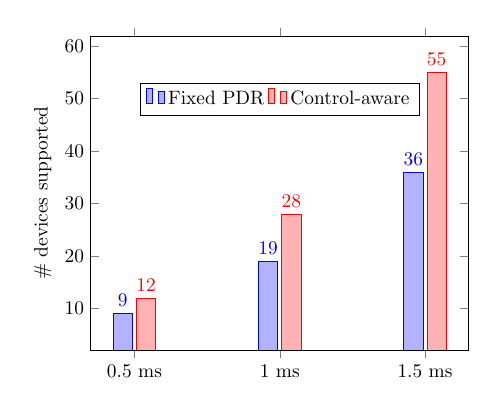
\begin{tikzpicture}[scale=0.7]
\begin{axis}[
    ybar,
    enlargelimits=0.15,
    legend style={at={(0.5,0.85)},
      anchor=north,legend columns=-1},
    ylabel={\# devices supported},
    symbolic x coords={0.5 ms,1 ms,1.5 ms},
    xtick=data,
    nodes near coords,
    nodes near coords align={vertical},
    ]
\addplot coordinates {(0.5 ms,9) (1 ms,19) (1.5 ms,36)};
\addplot coordinates {(0.5 ms,12) (1 ms,28) (1.5 ms,55)};
\legend{Fixed PDR, Control-aware}
\end{axis}
\end{tikzpicture} 
\caption{Simulation results for a series of inverted pendulums controlled over shared wireless channel. (left) The average distances from center vertical for $m=25$ pendulums. The control-aware, or ``co-design'', scheduler keeps all pendulums close, unlike the fixed PDR scheduler. (right) For different latency bounds, the control-aware can support more pendulums than the fixed PDR scheduler.}\label{fig_sim_results}
\end{figure*}


Given the set of devices selectively scheduled via \eqref{eq)prob_c}, we proceed to discuss an assignment-based formulation that can be employeed to select a low-latency schedule. Define the set of $m_k$ devices to selected be scheduled as $\ccalI_k \subseteq \{1,2,\hdots,m\}$ where  $| \ccalI_k| = m_k$ and device $j \in \ccalI_k$ with probability $\nu_{i,k}$. Further define $\ccalS_{(n)} \subset \ccalS$ to be an arbitrary set of $n$ FDs that do not intersect over any frequency bands, i.e. $\sum_{j \in \ccalS_{(n)}} \bbsigma_j \leq \mathbf{1}$. To accommodate the $m_k$ devices to be scheduled, we consider a set of $S$ such sets  $\{\ccalS^s_{(n_s)}\}_{s=1}^S$ with size $n_s$, whose combined elements total $\sum_{s=1}^{S} n_s = m_k$. We define this full set of assignable FDs at cycle $k$ as
%
\begin{align}\label{eq_ru_sets}
\ccalS'_k :=\ccalS^1_{(n_1)} \cup \ccalS^1_{(n_2)} \cup \hdots \cup \ccalS^{S_k}_{(n_{S_k})}.
\end{align}
%
Observe that an FD $\bbsigma$ is further superindexed by its TD slot $s$ y. In this way \eqref{eq_ru_sets} defines a complete set of  combinations of frequency-allocated FD and \emph{time}-allocated TDs to assign users during this cycle. An example of a possible $\ccalS'_k$ for scheduling $m_k = 12$ devices is shown in Table \ref{tab_rus}. 



For all $i \in \ccalI_k$ and FD $\bbsigma \in \ccalS'_k$, define the largest affordable DR given the \emph{modified} PDR requirement $\tdq_i(\hbx^{(l_i)}_{i,k})/\nu_{i,k}$ by
 %
 \begin{align}\label{eq_mcs_select}
 \mu_{i,k}(\bbsigma) := \begin{cases}
 \max \{\mu \mid q(\bbh_{i,k},\mu,\bbsigma) \geq \tdq_i(\hbx^{(l_i)}_{i,k})/\nu_{i,k}\} \\
 \mu_0,\quad  \text{ if } q(\bbh_{i,k},\mu,\bbsigma) < \tdq_i(\hbx^{(l_i)}_{i,k})/\nu_{i,k} \ \forall \mu
 \end{cases}
 \end{align}
 %
Observe in \eqref{eq_mcs_select} that, when no DR achieves the desired PDR in a particular FD, this value is set to $\mu=\mu_0$ by default.  The DR defined in \eqref{eq_mcs_select} subsequently incurs a time cost $\tau(\mu_{i,k}(\bbsigma), \bbsigma)$ for assigning device $i$ to FD $\bbsigma$. Define an \emph{assignment} $\ccalV=\{v_{ij}^s\}$ that assigns each device $i \in \ccalI_k$ to an FD/TD pair $(j,s)$ corresponding to an element in $\ccalS'_k$.  For time sensitive applications, the goal is to minimize the total transmission time across all TDs. The transmission time of a single TD is limited by the slowest device (i.e. a TD cannot finish until all devices finish transmitting). Thus, we can write the total transmission time as 
%
\begin{align}\label{eq_assignment}
T(\ccalV) = \sum_{s=1}^S \max_{j} \left[v^s_{ij} \tau(\mu_{i,k}(\bbsigma^s_j), \bbsigma_j^s)\right].
\end{align}
% 
The problem of minimizing $T(\ccalV)$ is a particular version of a non-linear assignment problem, where the goal is to choose an assignment---or schedule---that minimizes transmission time while meeting the control-aware PDR targets in \eqref{eq_pdr_constraint}. These problems are combinatorial in nature and challenging to solve exactly. We may approximate this problem by applying, e.g., the Hungarian method \cite{kuhn1955hungarian}, a well-known method for solving linear-cost assignment problems. Other heuristic assignment approaches may be designed to approximate the solution to \eqref{eq_assignment}. For the simulations performed later in this paper, we apply such a heuristic method, the details of which are left out for proprietary reasons.




The complete control-aware scheduling procedure for low-latency settings is present in Algorithm \ref{alg_calls}. At each cycle $k$, the BS uses current channel states $\bbh_{i,k}$ (obtained via pilot signals) and the current estimated control states $\hbx^{(l_i)}_{i,k}$  (obtained via \eqref{eq_state_est} for each device $i$) to compute control-aware target PDRs  $\tdq_i(\hbx^{(l_i)}_{i,k})$ for each device via \eqref{eq_pdr_constraint} in Step 3. In Step 4, the target PDRs are used to establish selection probabilities $\nu_{i,k}$ for each agent with \eqref{eq_prob_c}. After randomly selecting devices $\ccalI_k$ in Step 5, an appropriate set of FDs and TDs $\ccalS'_k$ are selected in Step 6. In Step 7, the associated DR values are determined for each possible assignment of device to FDs via \eqref{eq_mcs_select}. Finally, in Step 8 the assignment is performed using, e.g., the Hungarian method or other user-designed heuristic assignment method. The resulting assignment determines the scheduling parameters $\{\bbsigma_i, \mu_i, \alpha_i\}$ for all devices $i$ in the current cycle. 
 

 \begin{figure*}[t]
\centering
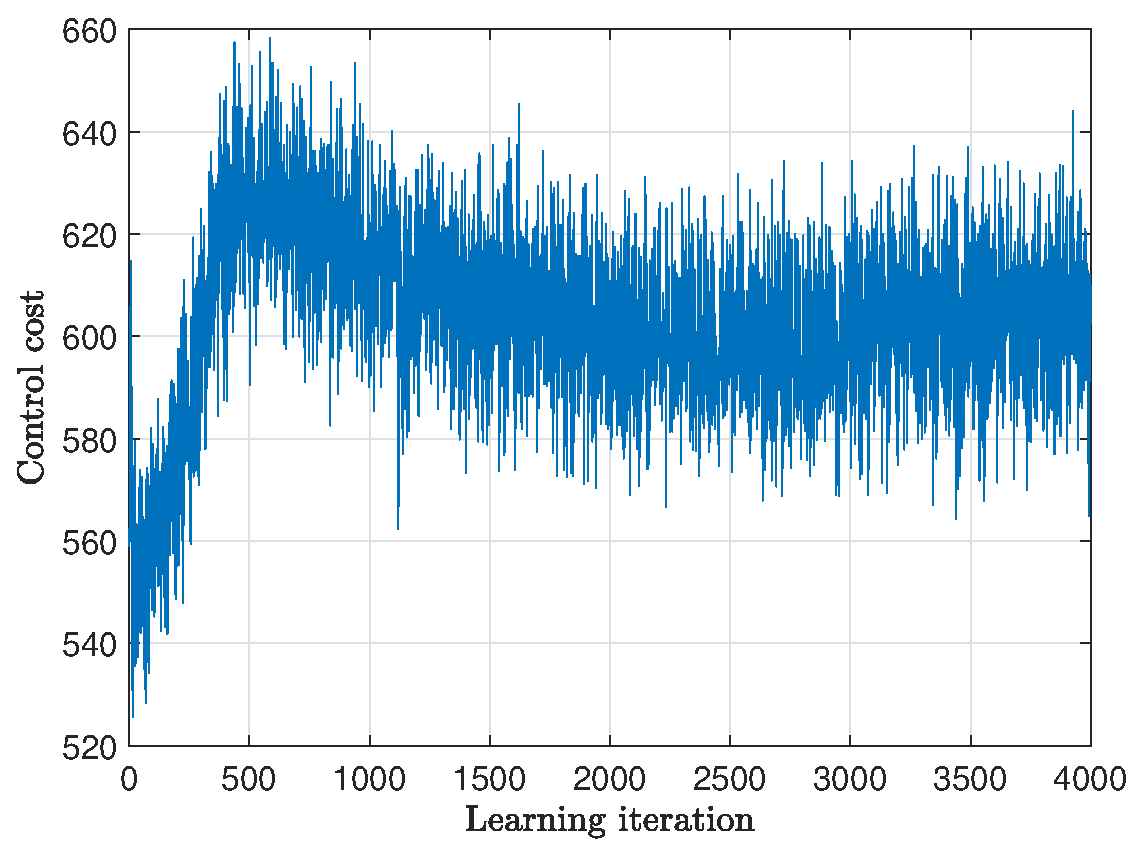
\includegraphics[width=0.45\linewidth, height=.18\textheight, keepaspectratio]{../images/cost_plot.eps} \qquad
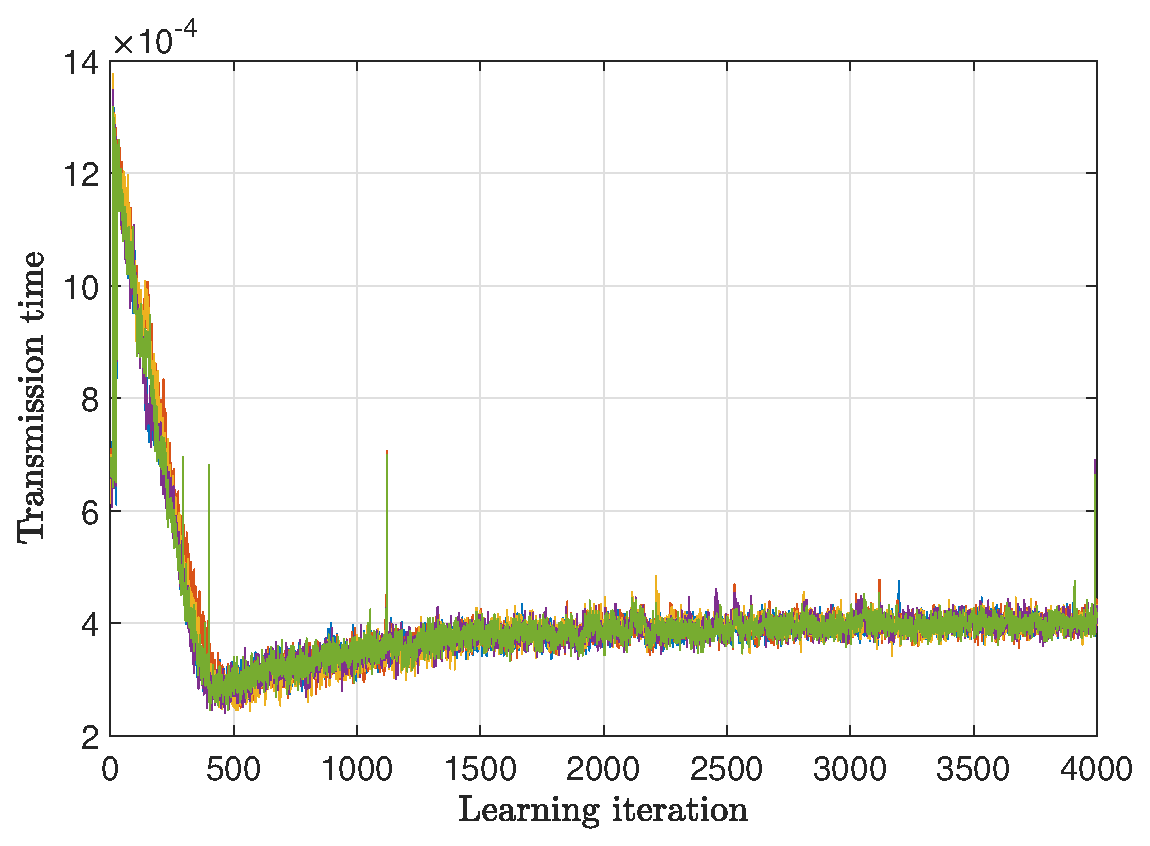
\includegraphics[width=0.45\linewidth, height=.18\textheight, keepaspectratio]{../images/time_plot.eps} 
\caption{Convergence of (left) objective function value, and (right) transmission time for a low-latency, control aware scheduling policy over the learning process. The DNN parameterized scheduling policy obtains feasible latency-contained schedules ($t_{\max} = 5 \times 10^{-4}$) that converges to a local minimum.}\label{fig_simple_results}
\end{figure*}

 %%%%%%%%%%%%%%%%%%%%%%%%%%%%%%%%%%%%%%%%%%%%%%%%%%%%%%%%%%%%%%%%%%%%
%%%   S   E   C   T   I   O   N   %%%%%%%%%%%%%%%%%%%%%%%%%%%%%%%%%%
%%%%%%%%%%%%%%%%%%%%%%%%%%%%%%%%%%%%%%%%%%%%%%%%%%%%%%%%%%%%%%%%%%%%
 
 \section{Simulation Results}\label{sec_numerical_results}
 

 
We perform a series of simulations on latency-constrained wireless control systems to evaluate the performance the learning method in and the resulting control-aware scheduling policies. We generate a series $m=20$ plants with closed-loop gains $\hbA_i \sim \text{Uniform}(0.8,0.95)$ and open-loop gains $\mathring{\bbA}_i \sim \text{Uniform}(1.01,1.3)$. The variance for all system noise $\bbw_i$ is set to be $W=1$. All such plants send their state information over a shared wireless channel with $n=5$ independent channels with a total latency constraint of $t_{\max} = 0.5$ ms. A latency bound of this order is typical of industrial control systems such as printing machines and presses \cite{ashraf2016ultra}. We further assume that the states of the plants are confined to the box $[-10,10]$. The DNN is given an architecture of 4 layers of sizes 256, 128, 64, and 32, all using a ReLU activation function.

With the scheduling architecture given in Figure \ref{fig_multi} for 5 channels and 20 plants, at each control scheduling interval each plant is given a data rate $\mu_i$ and a set of channels to transmit on. In our simulations, we use the modulation and coding schemes (MCS) of the next-generation IEEE 802.11ax Wi-Fi protocol as a representative architecture for data rate selection and packet error rate computation. As such, the continuous data rates $\mu_i$ are selected in an interval of $[1.6, 8]$ and rounded down to the nearest discrete MCS selection given in 802.11ax---see \cite{liu2014ieee} for details on the MCS tables given in this protocol. The corresponding transmission time $\tau(\mu)$ is then calculated assuming a fixed packet size of 100 bytes and the packet delivery rate $q(h,\mu)$ is computed using the associated AWGN error curve (scaled by the effective SNR given channel conditions).



 \begin{figure}
\centering
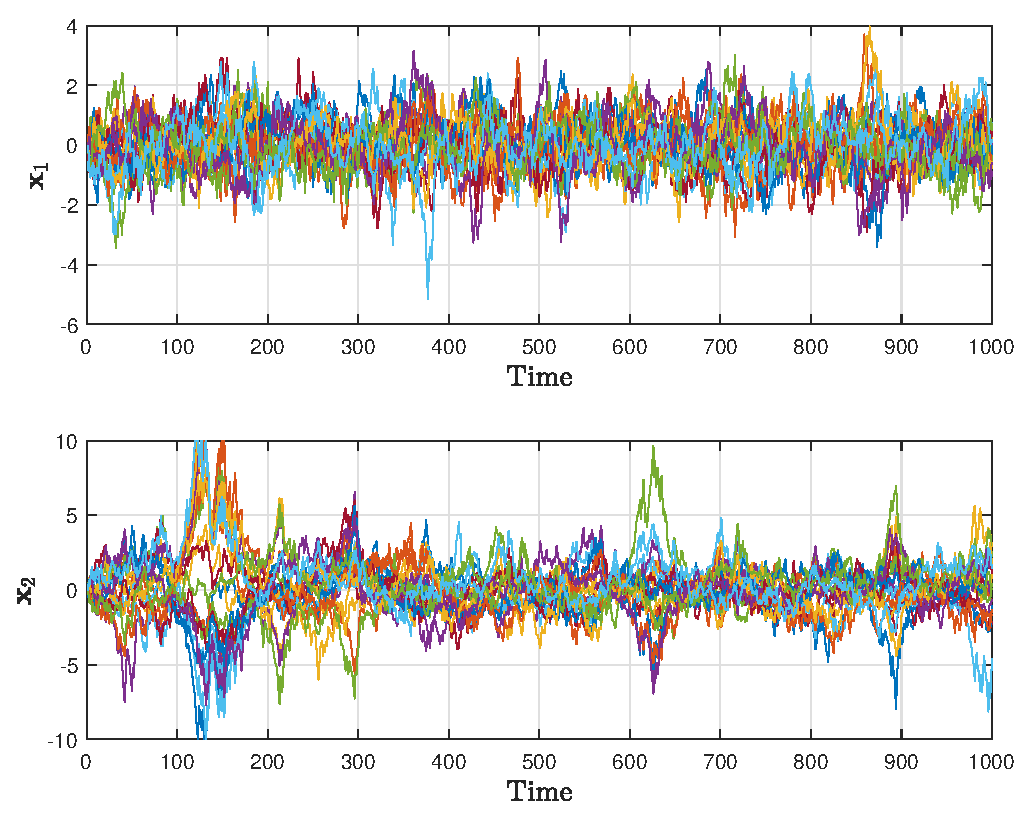
\includegraphics[height=.22\textheight]{../images/system_simulation.eps}
\caption{Evolution of plant states over 1000 control cycles using both the (top) DNN-based control aware scheduler and (b) a round robin scheduler.}\label{fig_system}
\end{figure}

In Figure \ref{fig_simple_results} we show the training process for the control-aware scheduler using the primal-dual scheduler given in Algorithm \ref{alg:learning}. In the left figure, we show the aggregate Lyapunov control cost over the course of $40,000$ learning iterations and in the right figure, show the transmission time of each channel (shown in different colored lines). As can be seen the in the figure, the policies initially output infeasible schedules that are beyond the latency limit but eventually converge to scheduling decisions that respect latency requirements. The control objective continues to decrease after feasibility is obtained and eventually converges to a local minimum value.


We proceed to simulate the performance of the control systems using the scheduling policy obtained at the end of the learning process and compare against a standard, round-robin scheduling policy---i.e. control-agnostic. Because the constraint in \eqref{eq_problem} is satisfied only with probability $1-\delta$, we ensure latency requirements are met at runtime by restricting all transmissions that are scheduled after the latency bound. In Figure \ref{fig_system} we show the state values over 1000 control cycles for the DNN-based scheduler (top figure) and the round robin scheduler (bottom figure). It can be observed that, overall, the plants are kept in better states using the DNN scheduler than with the round robin scheduler. This representative simulation highlights the ability of control-aware scheduling to better meet strict latency demands and, furthermore, highlight the ability of a DNN to properly encode such a constraints and objective in its dense architecture. 



 %%%%%%%%%%%%%%%%%%%%%%%%%%%%%%%%%%%%%%%%%%%%%%%%%%%%%%%%%%%%%%%%%%%%
%%%   S   E   C   T   I   O   N   %%%%%%%%%%%%%%%%%%%%%%%%%%%%%%%%%%
%%%%%%%%%%%%%%%%%%%%%%%%%%%%%%%%%%%%%%%%%%%%%%%%%%%%%%%%%%%%%%%%%%%%
 
 \section{Conclusion}
In this paper we develop a control-communication control-aware approach towards scheduling for low-latency wireless control systems. To handle the challenge of achieving high reliability performance with limited scheduling resources, we formulate a control-aware scheduling problem in which reliability is adapted to control and channel states and plant dynamics. This problem takes the form of a constrained statistical learning problem, in which solutions can be found by parameterized the scheduling policy with a deep neural network and applying a primal-dual learning framework to obtain the optimal weights of the neural network. Numerical simulations showcase the ability of the primal-dual method to find scheduling policies that outperform simple control-agnostic scheduling procedures.



% References should be produced using the bibtex program from suitable
% BiBTeX files (here: strings, refs, manuals). The IEEEbib.bst bibliography
% style file from IEEE produces unsorted bibliography list.
% -------------------------------------------------------------------------
\urlstyle{same}
\bibliographystyle{../IEEEbib}
\bibliography{../wireless_ll_control,../scheduling_control}


\end{document}